\subsubsection{Pagina principala}

\vspace{1cm}
\begin{center}
	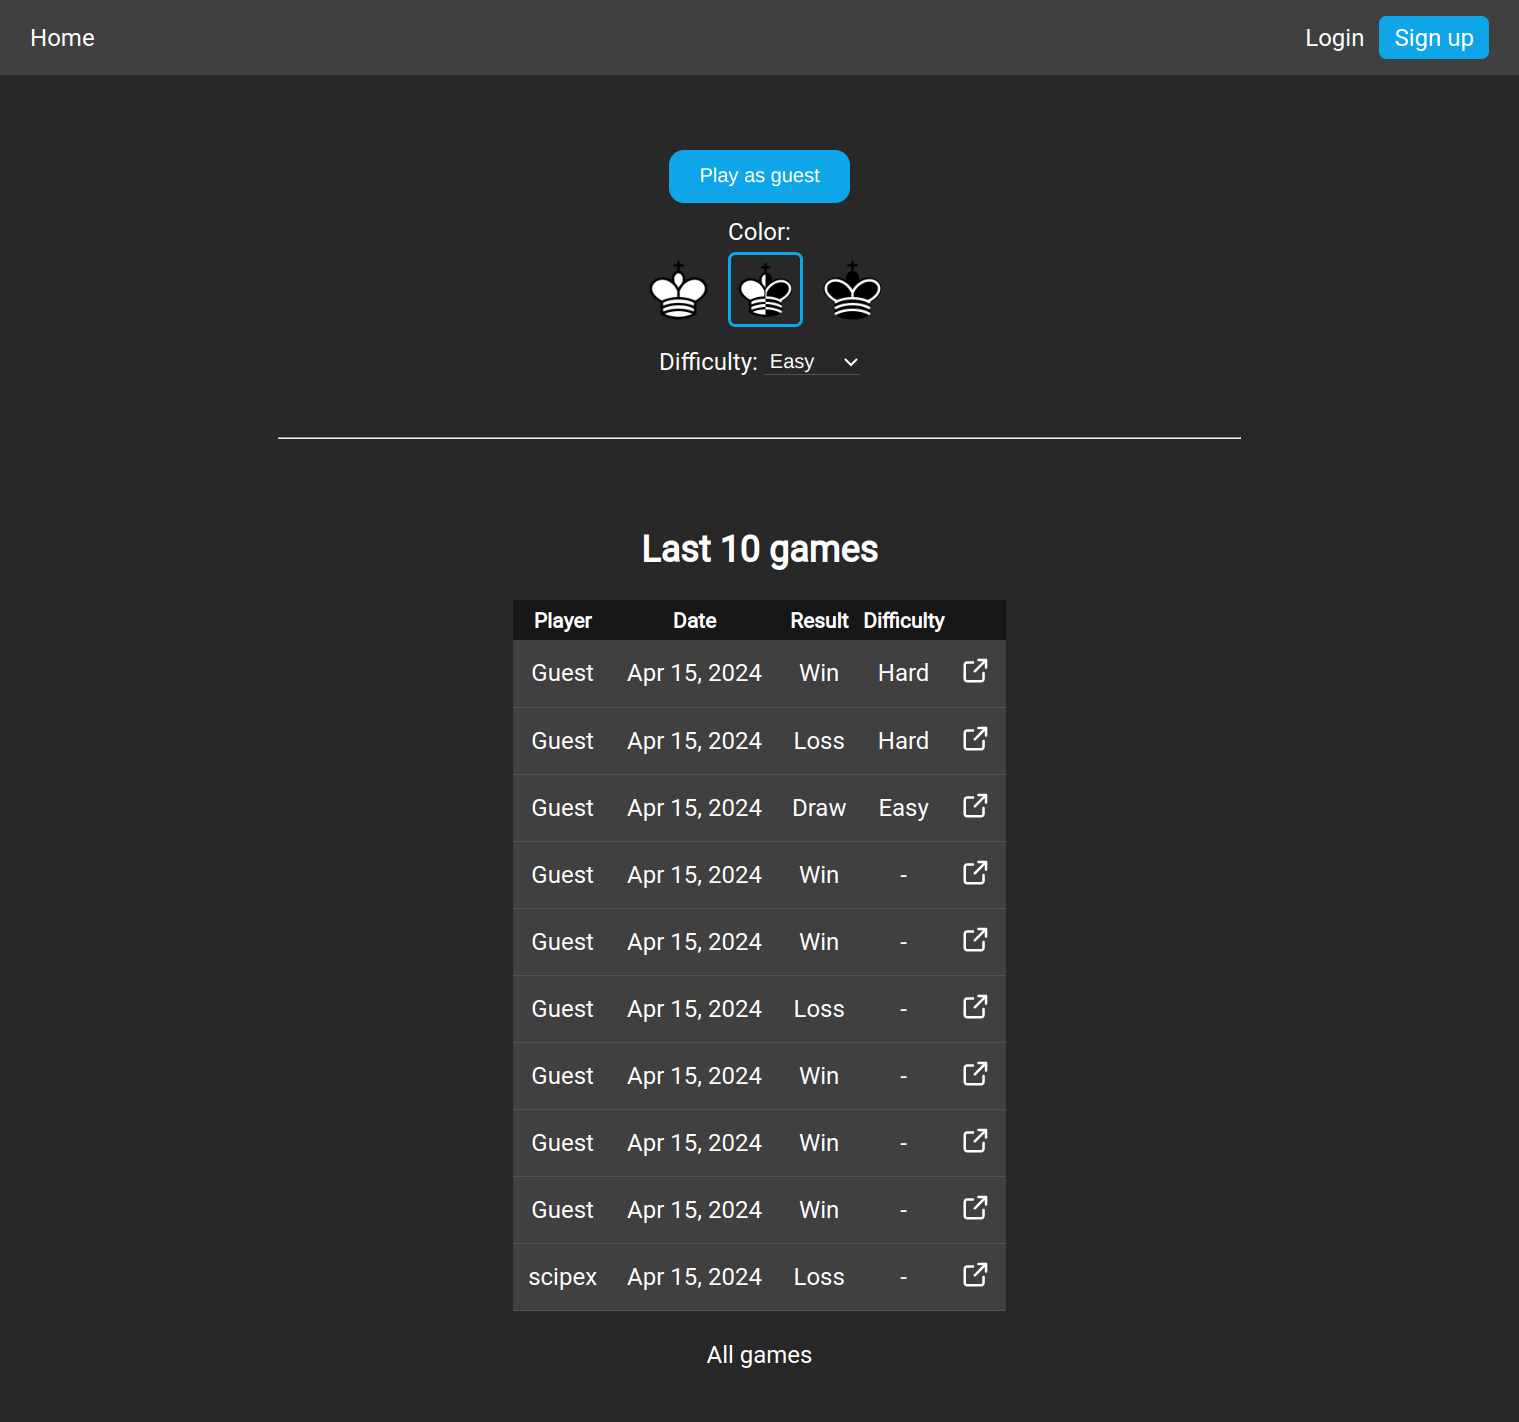
\includegraphics[width=15cm]{3/frontend/homepage.png}
\end{center}
\vspace{1cm}

Această pagină conține mai multe elemente:
\begin{itemize}
	\item Bara de navigație, prezentă pe toate paginile cu un link către pagina
	      principală în partea stângă, iar în partea dreaptă linkuri pentru
	      înregistrare/autentificare, dacă utilizatorul nu este autentificat,
	      sau un link pentru deconectare și unul pentru vizitarea profilului, dacă
	      utilizatorul este autentificat

	      \begin{lstlisting}[language=RustHtml]
fn navbar(user: Option<User>) -> String {
    html!(
        <div class="navbar-wrapper">
            <div class="navbar">
                <a href="/">"Home"</a>

                <div class="user">
                    {match user {
                        Some(user) => logged_in(user),
                        None => not_logged_in(),
                    }}
                </div>
            </div>
        </div>
    )
}

fn logged_in(user: User) -> String {
    html!(
        <a href="/logout" class="login">"Logout"</a>
        <a href={format!("/users/{}", &user.username)} class="profile">{&user.username}</a>
    )
}

fn not_logged_in() -> String {
    html!(
        <a href="/login" class="login">"Login"</a>
        <a href="/register" class="register">"Sign up"</a>
    ) 
}
\end{lstlisting}

	\item Meniu pentru începerea unui nou joc, realizat printr-un form HTML

	      \begin{lstlisting}[language=RustHtml]
fn new_game(button_text: &str) -> String {
    html!(
        <form action="/new-game" class="gameopts">
            <button class="newgame" type="submit">{button_text}</button>
            <div class="coloropt">
                <p style="margin: 0">"Color:"</p>
                <div style="display: flex">
                    {color_select("white", "checked")}
                    {color_select("random", "")}
                    {color_select("black", "")}
                </div>
            </div>
            <div class="divopt">
                <p style="margin: 0">"Difficulty:"</p>
                <select name="difficulty" class="difficulty">
                    <option value="0">"Easy"</option>
                    <option value="1">"Medium"</option>
                    <option value="2">"Hard"</option>
                </select>
            </div>
        </form>
    )
}

fn color_select(color: &str, checked: &str) -> String {
    html!(
        <div class="tooltip">
            <input type="radio" name="color" id=color value=color style="appearance: none" {checked} />
            <label for=color>
                <img class="colorselect" src=format!("/assets/select-{}.png", color) />
            </label>
            <span class="tooltiptext">{color}</span>
        </div>
    )
}
\end{lstlisting}

	\item Tabel cu ultimele 10 jocuri

	      Generat pe server

	      \begin{lstlisting}[language=RustHtml]
pub fn games_list(games: Vec<Game>) -> String {
    html! {
        <table class="games">
            <tr class="games-header">
                <th style="padding: 5px 0px;">"Player"</th>
                <th>"Date"</th>
                <th>"Result"</th>
                <th>"Difficulty"</th>
                <th></th>
            </tr>
            {games.into_iter().map(game_html).collect::<String>()}
        </table>
    }
}
\end{lstlisting}

	      \begin{lstlisting}[language=RustHtml]
pub fn game_html(game: Game) -> String {
    let date_format = time::format_description::parse("[month repr:short] [day], [year]").unwrap();
    let date = game.played_at.format(&date_format).unwrap().to_string();
    let difficulty = game.difficulty.clone().unwrap_or("-".into());

    html! {
        <tr class="game" onclick={format!("location.href='/games/{}';", game.id)}>
            <td>{player(&game)}</td>
            <td>{date}</td>
            <td>{game.result}</td>
            <td>{difficulty}</td>
        </tr>
    }
}

fn player(game: &Game) -> String {
    match &game.player {
        Some(player) => html! {
            <a class="player" href={format!("/users/{}", player)}>{player}</a>
        },
        None => html! {
            "Guest"
        },
    }
}
\end{lstlisting}
\end{itemize}
